\chapter{Introduzione}

Alla fine del 1700, quella che veniva chiamata "Filosofia naturale" iniziò a scindersi in due grandi ambiti di studio:
\begin{itemize}
    \item \textbf{Scienze Biologiche}: dedicate allo studio degli esseri viventi.
    \item \textbf{Scienze Fisiche}: dedicate allo studio della materia inanimata.
\end{itemize}
All'interno delle scienze fisiche, si consolidò ulteriormente la distinzione tra:
\begin{itemize}
    \item \textbf{Chimica}: che studia la formazione e la trasformazione delle molecole.
\end{itemize}

\begin{definizione}{Fisica}
La Fisica (dal greco \emph{physis}, "natura") è una \textbf{scienza sperimentale} in continua evoluzione che indaga i costituenti fondamentali della materia e le loro interazioni attraverso il \textbf{Metodo Scientifico}. Si occupa dei fenomeni naturali, sia quelli "reali" (osservati in natura) che quelli "riprodotti" (in laboratorio).
\end{definizione}

\vspace{0.5cm}

\begin{figure}[ht]
\centering
\begin{tikzpicture}[scale=0.65, transform shape,
    node distance=1.5cm,
    auto,
    block/.style={rectangle, draw, fill=blue!8, text width=10em, text centered, rounded corners=3pt, minimum height=4em, thick},
    decision/.style={diamond, aspect=2, draw, fill=yellow!15, text width=5em, text centered, inner sep=2pt, thick},
    outcome/.style={rectangle, draw, thick, text width=9em, text centered, rounded corners=3pt, minimum height=3.5em},
    arrow/.style={->, >=stealth, thick, draw=gray!80}
]
    % Nodes aligned vertically
    \node [block] (osserv) {Osservazione};
    \node [block, below=of osserv] (riprod) {Riproduzione Semplificata\\(Esperimento)};
    \node [block, below=of riprod] (dati) {Raccolta Dati};
    \node [block, below=of dati] (interp) {Interpretazione\\(Teoria)};
    
    \node [decision, below=1.8cm of interp] (verifica) {Conferma?};

    % Outcomes (closer to diamond as requested)
    \node [outcome, right=1.5cm of verifica, fill=green!15] (tesi) {Tesi Confermata};
    \node [outcome, left=1.5cm of verifica, fill=red!15] (crisi) {Crisi\\(Correzioni)};

    % Edges
    \draw [arrow] (osserv) -- (riprod);
    \draw [arrow] (riprod) -- (dati);
    \draw [arrow] (dati) -- (interp);
    \draw [arrow] (interp) -- (verifica);
    
    \draw [arrow] (verifica) -- node [above, near start] {\small SÌ} (tesi);
    \draw [arrow] (verifica) -- node [above, near start] {\small NO} (crisi);
    
    % Feedback loop: detached from lilac blocks, reconnecting from the left to the first light block
    \draw [arrow, rounded corners=15pt] (crisi.west) -- ++(-1.5,0) |- node [pos=0.25, left, rotate=90, anchor=south] {\small Nuova Ipotesi} (osserv.west);

\end{tikzpicture}
\caption{Schema del Metodo Scientifico: un processo ciclico di verifica.}
\label{fig:metodo}
\end{figure}

\newpage

\section{Il Metodo Scientifico Sperimentale}

Il metodo scientifico è il pilastro dell'indagine fisica. È un ciclo continuo che permette di validare o confutare le teorie.
Partendo dall'\textbf{osservazione} di un fenomeno, si tenta una \textbf{riproduzione semplificata} (esperimento) per raccogliere \textbf{dati}. L'\textbf{interpretazione} di questi dati porta alla formulazione di una \textbf{teoria}. Se la teoria viene verificata sperimentalmente, diventa una tesi confermata; altrimenti, si entra in una fase di crisi che richiede correzioni o nuove ipotesi (vedi Fig. \ref{fig:metodo}).



\section{Evoluzione delle Branche della Fisica}

La Fisica si è evoluta storicamente passando dalla visione classica a quella moderna, spinte dalla necessità di spiegare fenomeni sempre più complessi o estremi.

\begin{figure}[ht]
\centering
\begin{tikzpicture}[scale=0.85, transform shape,
    box_classica/.style={rectangle, draw=black, thick, fill=orange!15, text width=3.8cm, text centered, rounded corners=3pt, minimum height=1.2cm},
    box_moderna/.style={rectangle, draw=black, thick, fill=cyan!15, text width=3.8cm, text centered, rounded corners=3pt, minimum height=1.2cm},
    box_ponte/.style={rectangle, draw=black, thick, fill=yellow!25, text width=4cm, text centered, rounded corners=3pt, minimum height=1.8cm},
    header/.style={font=\bfseries\large},
    label_style/.style={font=\itshape\small},
    arrow/.style={->, >=stealth, line width=2pt, draw=gray!60}
]

    % Column Headers
    \node[header] at (0, 1) {FISICA CLASSICA};
    \node[header] at (10, 1) {FISICA MODERNA};

    % Classica Nodes
    \node[box_classica] (mecc) at (0, 0) {Meccanica};
    \node[box_classica] (termo) at (0, -1.5) {Termodinamica};
    \node[box_classica] (acus) at (0, -3) {Acustica};
    \node[box_classica] (ott) at (0, -4.5) {Ottica};

    % Moderna Nodes
    \node[box_moderna] (rel) at (10, 0) {Relatività};
    \node[box_moderna] (atom) at (10, -1.5) {Fisica Atomica};
    \node[box_moderna] (nucl) at (10, -3) {Fisica Nucleare};
    \node[box_moderna] (sub) at (10, -4.5) {Fisica Subnucleare};

    % Ponte Elettromagnetismo (Vertically aligned with column centers at -2.25)
    \node[box_ponte] (em) at (5, -2.25) {Elettromagnetismo\\($\vec{E}, \vec{B}$)};
    
    % Passaggio Text (outside box, stylized)
    \node[below=0.3cm of em, label_style] {\textit{Passaggio}};

    % Clean, straight, centered arrows in the gaps
    % Gap Left: mecc.east (x=1.9) to em.west (x=3.0). Gap = 1.1cm.
    % We draw arrow from x=2.1 to x=2.8.
    \draw [arrow] (2.1, -2.25) -- (2.8, -2.25);

    % Gap Right: em.east (x=7.0) to rel.west (x=8.1). Gap = 1.1cm.
    % We draw arrow from x=7.2 to x=7.9.
    \draw [arrow] (7.2, -2.25) -- (7.9, -2.25);

\end{tikzpicture}
\caption{Lo sviluppo storico dalla Fisica Classica alla Moderna.}
\end{figure}

Dalla \textbf{Meccanica Newtoniana} (o Classica), valida per velocità basse rispetto alla luce ($v \ll c$) e dimensioni umane, si è passati a nuove teorie per spiegare gli estremi:
\begin{itemize}
    \item \textbf{Relatività Ristretta e Generale}: necessarie per velocità prossime a ($c$) o forti campi gravitazionali.
    \item \textbf{Meccanica Quantistica}: necessaria per descrivere il comportamento della materia su scala atomica ($L \sim$ atomo).
\end{itemize}

Inoltre, esiste un legame circolare tra \textbf{Fisica e Tecnologia}: la fisica ispira nuove tecnologie, e le nuove tecnologie forniscono strumenti più precisi per fare nuova fisica (es. acceleratori di particelle, laser, semiconduttori).

\section{La Misurazione}
\begin{definizione}{Misurazione}
La misurazione è il processo di confronto di una grandezza fisica con un'unità di misura predefinita. Poiché è impossibile ottenere un valore "esatto", il risultato si esprime come:
\[ x \pm \delta x \]
\end{definizione}

Le cause di incertezza possono essere:
\begin{itemize}
    \item \textbf{Variabilità del campione}.
    \item \textbf{Errore Sistematico}: precisione dello strumento.
    \item \textbf{Errore Accidentale}: fluttuazione delle misure ripetute sullo stesso campione.
\end{itemize}

\begin{esercizio}{Propagazione dell'Errore: Esempio Geometrico}
Un errore può propagarsi attraverso i calcoli, rendendo la determinazione dell'incertezza $\delta x$ complessa.
Consideriamo l'esempio semplice dell'area di un rettangolo misurato.

    \begin{center}
    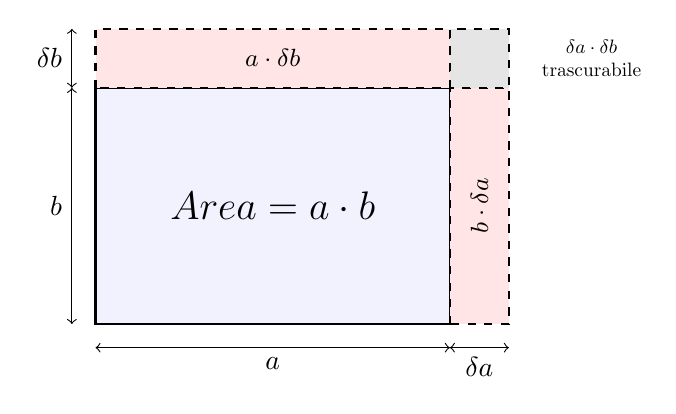
\begin{tikzpicture}[scale=1.5]
        % Rettangolo Principale A = ab
        \draw[thick, fill=blue!5] (0,0) rectangle (3,2);
        \node at (1.5,1) {\Large $Area = a \cdot b$};
        
        % Striscia errore altezza (a * delta b)
        \draw[thick, dashed, fill=red!10] (0,2) rectangle (3,2.5);
        \node at (1.5, 2.25) {\small $a \cdot \delta b$};
        
        % Striscia errore base (b * delta a)
        \draw[thick, dashed, fill=red!10] (3,0) rectangle (3.5,2);
        \node[rotate=90] at (3.25, 1) {\small $b \cdot \delta a$};
        
        % Angolo trascurabile (delta a * delta b)
        \draw[thick, dashed, fill=gray!20] (3,2) rectangle (3.5,2.5);
        \node[scale=0.7, align=center] at (4.2, 2.25) {$\delta a \cdot \delta b$\\trascurabile};
        
        % Quote
        \draw[<->] (0,-0.2) -- (3,-0.2) node[midway, below] {$a$};
        \draw[<->] (3,-0.2) -- (3.5,-0.2) node[midway, below] {$\delta a$};
        
        \draw[<->] (-0.2,0) -- (-0.2,2) node[midway, left] {$b$};
        \draw[<->] (-0.2,2) -- (-0.2,2.5) node[midway, left] {$\delta b$};
    \end{tikzpicture}
    \captionof{figure}{Propagazione dell'errore nel calcolo dell'Area ($A \pm \delta A$).}
    \label{fig:errore_area}
    \end{center}

Se misuriamo i lati come $a \pm \delta a$ e $b \pm \delta b$, l'area calcolata sarà:
\[
A_{mis} = (a \pm \delta a)(b \pm \delta b) = \underbrace{ab}_{A} \pm \underbrace{a\delta b \pm b\delta a}_{\delta A} + \underbrace{\delta a \delta b}_{\approx 0}
\]
Poiché $\delta a \ll a$ e $\delta b \ll b$, il termine quadratico $\delta a \delta b$ è trascurabile. L'errore assoluto sull'area è quindi:
\[ \delta A \approx a\delta b + b\delta a \]
\end{esercizio}

\subsection{Rappresentazione dei Dati ed Errori}
A questo proposito introduciamo i concetti di:
\begin{itemize}
    \item \textbf{Cifra Significativa (CF)}: Indica la precisione della misura (es. misurare $3,0$ è diverso da misurare $3$, in quanto indica una precisione decimale).
    \item \textbf{Notazione Scientifica (NS)}: Si usa la forma $x \cdot 10^n$ per scrivere numeri molto grandi o piccoli mantenendo chiare le cifre significative.
\end{itemize}

L'errore può essere classificato come:
\begin{itemize}
    \item \textbf{Assoluto} ($x \pm \delta x$): Ha la stessa unità di misura della grandezza.
    \item \textbf{Relativo} ($x \pm \frac{\delta x}{|x|}$): È un numero puro (spesso espresso in \%).
\end{itemize}

\begin{definizione}{Grandezza Fisica}
La definizione di una grandezza fisica si dice \textbf{operativa}, poiché elenca le procedure da compiere per misurarne la quantità attraverso il confronto con un'\textbf{Unità di Misura} (UdM). Se le grandezze a confronto non sono della stessa specie (\textbf{non omogenee}), si opera una equivalenza tramite un \textbf{fattore di ragguaglio}.
\end{definizione}

Discende quindi la distinzione tra:
\begin{itemize}
    \item \textbf{Grandezze Fondamentali} (o Primitive): Misurate per via \textbf{diretta}.
    \item \textbf{Grandezze Derivate}: Misurate per via \textbf{indiretta} (tramite relazioni matematiche tra grandezze primitive).
\end{itemize}

Nel Sistema Internazionale (SI), le \textbf{Grandezze Fondamentali} sono 7:
\begin{enumerate}
    \item \textbf{Lunghezza} ($m$, metro).
    \item \textbf{Massa} ($kg$, chilogrammo) - misurata con bilancia o spettrometro di massa.
    \item \textbf{Tempo} ($s$, secondo) - misurato con orologio.
    \item \textbf{Temperatura} ($K$, Kelvin) - misurata con termometro.
    \item \textbf{Intensità di corrente} ($A$, Ampere) - misurata con amperometro.
    \item \textbf{Intensità luminosa} ($cd$, candela) - misurata con fotometro.
    \item \textbf{Quantità di sostanza} ($mol$, mole).
\end{enumerate}

\section{Sistemi di Unità di Misura}
Esistono diversi sistemi di unità di misura costituiti da grandezze primitive indipendenti tra loro. I principali sono:
\begin{itemize}
    \item \textbf{MKS}: Metro ($m$), Chilogrammo ($kg$), Secondo ($s$). È alla base del Sistema Internazionale (SI).
    \item \textbf{CGS}: Centimetro ($cm$), Grammo ($g$), Secondo ($s$). Usato spesso in chimica o elettromagnetismo teorico.
    \item \textbf{Pratico}: Metro ($m$), Chilogrammo-peso ($kg_p$), Secondo ($s$). In questo sistema la forza è fondamentale e la massa derivata.
\end{itemize}

Tutti questi sistemi sono caratterizzati da tre dimensioni fondamentali: Lunghezza $[L]$, Massa $[M]$ e Tempo $[T]$.

\begin{osservazione}{Rivoluzione della Metrologia (2019)}
Dal 2019, i campioni fisici materiali (come il cilindro di platino-iridio per il chilogrammo) sono stati definitivamente abbandonati. Le unità di misura sono ora definite esclusivamente in base a \textbf{costanti fondamentali della fisica} (es. costante di Planck $h$, velocità della luce $c$, carica elementare $e$), garantendo invarianza e riproducibilità universale indipendentemente dal luogo o dallo strumento.
\end{osservazione}

\section{Analisi Dimensionale}
L'analisi dimensionale permette di studiare le dimensioni fisiche di una grandezza e verificare la correttezza delle equazioni. Ogni grandezza $X$ può essere espressa come prodotto di potenze delle grandezze fondamentali:
\[ [X] = [L]^\alpha \cdot [M]^\beta \cdot [T]^\gamma \quad \text{con } \alpha, \beta, \gamma \in \mathbb{Q} \]

\paragraph{Principio di Omogeneità:} In un'equazione fisica $A = B + C$, tutti i termini devono avere le stesse dimensioni ($[A] = [B] = [C]$).
Se $\alpha=\beta=\gamma=0$, la grandezza si dice \textbf{adimensionale} (numero puro).

\begin{esercizio}{Il Pendolo Semplice}
Vogliamo determinare da quali grandezze fisiche dipende il **Periodo di oscillazione ($T$)** di un pendolo semplice.

    \begin{center}
    \begin{tikzpicture}
        % Ceiling
        \draw[thick] (-2,0) -- (2,0);
        \fill[pattern=north east lines] (-2,0) rectangle (2,0.2);
        
        % Vertical dashed line
        \draw[dashed] (0,0) -- (0,-3);
        
        % Pendulum string
        \draw[thick] (0,0) -- (1.5,-2.5) node[midway, right] {$l$};
        
        % Mass
        \draw[thick, fill=gray!30] (1.5,-2.5) circle (0.3cm) node[right=0.4cm] {$m$};
        
        % Arc angle
        \draw[->] (0,-1) arc (270:300:1);
        \node at (0.3,-1.2) {$\theta$};
        
        % Gravity vector
        \draw[->, thick] (-1.5, -1) -- (-1.5, -2) node[right] {$\vec{g}$};
    \end{tikzpicture}
    \captionof{figure}{Pendolo semplice di lunghezza $l$ e massa $m$.}
    \end{center}

Ipotizziamo che il periodo $T$ dipenda dalla massa $m$, dalla lunghezza del filo $l$ e dall'accelerazione di gravità $g$. Scriviamo una relazione di proporzionalità generica:
\[ T = k \cdot m^\alpha \cdot l^\beta \cdot g^\gamma \]
dove $k$ è una costante adimensionale. Analizziamo le dimensioni di ogni termine:
\begin{itemize}
    \item Periodo: $[T] = [T]^1$
    \item Massa: $[m] = [M]$
    \item Lunghezza: $[l] = [L]$
    \item Gravità ($m/s^2$): $[g] = [L][T]^{-2}$
\end{itemize}

Sostituiamo nell'equazione dimensionale:
\[ [M]^0 [L]^0 [T]^1 = [M]^\alpha \cdot [L]^{\beta+\gamma} \cdot [T]^{-2\gamma} \]

Per il principio di omogeneità, impostiamo il sistema:
\[
\begin{cases}
    \alpha = 0 \\
    \beta + \gamma = 0 \\
    -2\gamma = 1
\end{cases}
\implies \alpha = 0, \beta = 1/2, \gamma = -1/2
\]

Otteniamo così la legge del periodo:
\[ \boxed{T = k \sqrt{\frac{l}{g}}} \]
\textbf{Conclusione}: Il periodo è indipendente dalla massa e dipende solo dalla lunghezza del filo e dalla gravità locale.
\end{esercizio}

\section{Multipli e Sottomultipli}
Ecco una tabella completa dei prefissi utilizzati nel Sistema Internazionale per esprimere multipli (lettere maiuscole, tranne $k$, $h$, $da$) e sottomultipli (lettere minuscole).

\begin{table}[h]
    \centering
    \renewcommand{\arraystretch}{1.2}
    \begin{tabular}{llc | llc}
        \toprule
        \multicolumn{3}{c|}{\textbf{Multipli (Grandi)}} & \multicolumn{3}{c}{\textbf{Sottomultipli (Piccoli)}} \\
        \midrule
        \textbf{Prefisso} & \textbf{Simb.} & \textbf{Fattore} & \textbf{Prefisso} & \textbf{Simb.} & \textbf{Fattore} \\
        \midrule
        deca  & $da$ & $10^1$  & deci  & $d$ & $10^{-1}$ \\
        etto  & $h$  & $10^2$  & centi & $c$ & $10^{-2}$ \\
        chilo & $k$  & $10^3$  & milli & $m$ & $10^{-3}$ \\
        Mega  & $M$  & $10^6$  & micro & $\mu$ & $10^{-6}$ \\
        Giga  & $G$  & $10^9$  & nano  & $n$ & $10^{-9}$ \\
        Tera  & $T$  & $10^{12}$ & pico  & $p$ & $10^{-12}$ \\
        Peta  & $P$  & $10^{15}$ & femto & $f$ & $10^{-15}$ \\
        Exa   & $E$  & $10^{18}$ & atto  & $a$ & $10^{-18}$ \\
        \bottomrule
    \end{tabular}
    \caption{Tabella completa dei multipli e sottomultipli SI.}
    \label{tab:multipli}
\end{table}

\section{Recap: Legami cinematici tra posizione, velocità e accelerazione}

Abbiamo definito le relazioni di derivazione, adesso introduciamo quelle di integrazione.
Possiamo schematizzare i legami tra posizione $\vec{x}(t)$, velocità $\vec{v}(t)$ e accelerazione $\vec{a}(t)$ come segue:

\begin{center}
\begin{tikzpicture}[node distance=2.5cm, auto, >=stealth]
    \node (x) {$\vec{x}$};
    \node (v) [right=of x] {$\vec{v}$};
    \node (a) [right=of v] {$\vec{a}$};

    \draw[->] (x) to [bend left=30] node {$v = \frac{d\vec{x}}{dt}$} (v);
    \draw[->] (v) to [bend left=30] node {$a = \frac{d\vec{v}}{dt}$} (a);
    
    \draw[->] (a) to [bend left=30] node {$v = \int a \, dt$} (v);
    \draw[->] (v) to [bend left=30] node {$x = \int v \, dt$} (x);
\end{tikzpicture}
\end{center}

Possiamo suddividere un intervallo di tempo $\Delta t$ in molti intervalli $\delta t = t_{i+1} - t_i$. Inoltre, la velocità media nell'intervallo può essere approssimata come la media aritmetica delle velocità agli estremi:
\[ v_m(t_i, t_{i+1}) = \frac{x(t_{i+1}) - x(t_i)}{t_{i+1} - t_i} \approx \frac{v(t_{i+1}) + v(t_i)}{2} \]

Lo spazio percorso tra un istante $t_0$ e un istante $t_n$ è dato dalla somma degli spostamenti nei singoli intervallini:
\begin{align*}
x_n - x_0 &= x(t_n) - x(t_0) = [x(t_n) - x(t_{n-1})] + \dots + [x(t_1) - x(t_0)] \\
&= v_m(t_{n-1}, t_n)\delta t + \dots + v_m(t_0, t_1)\delta t \\
&\approx \sum_{i=0}^{n-1} \left[ \frac{v(t_{i+1}) + v(t_i)}{2} \right] \delta t
\end{align*}
Geometricamente, notiamo che il termine $\frac{v(t_i) + v(t_{i+1})}{2} \delta t$ corrisponde all'\textbf{Area del trapezio} sotteso dalla curva $v(t)$ nell'intervallo $[t_i, t_{i+1}]$.
Pertanto:
\[ x_n - x_0 \approx \sum \text{Aree trapezi} \]

Passando al limite per $\delta t \to 0$:
\[ x_n - x_0 = \lim_{\delta t \to 0} \sum_{i=0}^{n-1} \left( \frac{v(t_i) + v(t_{i+1})}{2} \right) \delta t = \int_{t_0}^{t_n} v(t) \, dt \]

\begin{figure}[h]
    \centering
    \begin{tikzpicture}[scale=0.8]
        % Axes
        \draw[->] (0,0) -- (6,0) node[right] {$t$};
        \draw[->] (0,0) -- (0,4) node[above] {$v(t)$};
        
        % Curve
        \draw[thick, blue] plot [smooth] coordinates {(0.5,1) (1.5,2.5) (3,2.8) (4.5,3.2) (5.5,3.5)};
        
        % Trapezoids
        \foreach \x/\y in {0.5/1, 1.5/2.5, 3/2.8, 4.5/3.2} {
            \draw[dashed] (\x,0) -- (\x, \y);
            \node[below] at (\x,0) {\tiny $t_{i}$}; % Placeholder indices
        }
        \draw[dashed] (5.5,0) -- (5.5, 3.5);
        
        % Pattern area
        \fill[pattern=north east lines, pattern color=gray!40] (1.5,0) -- (1.5,2.5) -- (3,2.8) -- (3,0) -- cycle;
        \draw (1.5,2.5) -- (3,2.8); % Top segment of trapezoid
        
        \node at (2.25, 1) {Area};
        \node[below] at (0.5,0) {$t_0$};
        \node[below] at (5.5,0) {$t_n$};
    \end{tikzpicture}
    \caption{Interpretazione geometrica dell'integrale come area sottesa al grafico.}
\end{figure}

In sintesi, le relazioni integrali fondamentali sono:

\begin{itemize}
    \item \textbf{Spostamento vettoriale}:
    \[ \Delta \vec{x} = \vec{x}(t_n) - \vec{x}(t_0) = \int_{t_0}^{t_n} \vec{v}(t) \, dt \]
    
    \item \textbf{Variazione di velocità vettoriale}:
    \[ \Delta \vec{v} = \vec{v}(t_n) - \vec{v}(t_0) = \int_{t_0}^{t_n} \vec{a}(t) \, dt \]
    
    \item \textbf{Spazio percorso (Ascissa Curvilinea)}:
    \[ \Delta S = S(t_n) - S(t_0) = \int_{t_0}^{t_n} |\vec{v}(t)| \, dt \]
    \textit{Nota: qui si integra il modulo della velocità (la velocità scalare istantanea).}
    
    \item \textbf{Variazione di velocità scalare}:
    \[ \Delta v = v(t_n) - v(t_0) = \int_{t_0}^{t_n} |\vec{a}(t)| \, dt \]
    \textit{Nota: analogamente, si considera il contributo del modulo dell'accelerazione.}
\end{itemize}

\section{Moti Rettilinei Fondamentali}

Prima di analizzare moti più complessi, definiamo i due pilastri della cinematica unidimensionale.

\subsection{Moto Rettilineo Uniforme (MRU)}
È il moto di un punto che percorre una traiettoria rettilinea con velocità $\vec{v}$ costante in modulo, direzione e verso.
\[ a = 0 \implies v(t) = \text{costante} \]
La sua legge oraria è rappresentata da una retta:
\[ x(t) = x_0 + v(t - t_0) \]

\subsection{Moto Rettilineo Uniformemente Accelerato (MRUA)}
È il moto di un punto che si muove lungo una retta con accelerazione $\vec{a}$ costante.
Le leggi del moto sono:
\begin{align}
    v(t) &= v_0 + a(t - t_0) \\
    x(t) &= x_0 + v_0(t - t_0) + \frac{1}{2}a(t - t_0)^2
\end{align}

\begin{osservazione}{Derivazione Formula di Torricelli}
La formula di Torricelli mette in relazione velocità e spazio percorso eliminando la dipendenza esplicita dal tempo. Si ottiene isolando l'intervallo di tempo $\Delta t$ dalla legge della velocità e sostituendolo nella legge della posizione.
Ponendo $\Delta t = (t - t_0)$ e $\Delta x = (x - x_0)$:
\begin{enumerate}
    \item Dalla (1): $\Delta t = \frac{v - v_0}{a}$
    \item Sostituiamo in (2): $\Delta x = v_0 \left( \frac{v - v_0}{a} \right) + \frac{1}{2} a \left( \frac{v - v_0}{a} \right)^2$
\end{enumerate}
Sviluppando i calcoli:
\[ \Delta x = \frac{v_0 v - v_0^2}{a} + \frac{1}{2} a \frac{(v - v_0)^2}{a^2} = \frac{v_0 v - v_0^2}{a} + \frac{v^2 - 2v v_0 + v_0^2}{2a} \]
Moltiplicando tutto per $2a$:
\[ 2a \Delta x = 2v_0 v - 2v_0^2 + v^2 - 2v v_0 + v_0^2 \]
\[ 2a \Delta x = v^2 - v_0^2 \implies \boxed{v^2 = v_0^2 + 2a \Delta x} \]
\end{osservazione}

\section{Altri Moti della Cinematica}
Oltre ai moti rettilinei uniformi e accelerati, la cinematica studia:
\begin{itemize}
    \item Moto vario accelerato
    \item Moto armonico (semplice, smorzato, forzato)
    \item Moto dei gravi (caduta libera e parabolico)
    \item Moti curvilinei (circolare, ellittico)
\end{itemize}

\section{Moto Armonico Semplice (MAS)}

Il moto armonico descrive i sistemi che oscillano attorno a una posizione di equilibrio stabile. A differenza del MRUA, nel moto armonico l'accelerazione \textbf{NON è costante}.

\subsection{Funzioni Periodiche vs Armoniche}
È fondamentale distinguere tra una funzione periodica generica e una funzione armonica.

\begin{figure}[ht]
    \centering
    \begin{minipage}{0.48\textwidth}
        \centering
        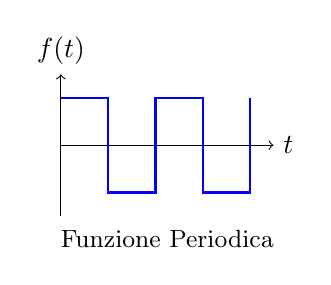
\begin{tikzpicture}[scale=0.6]
            \draw[->] (0,0) -- (4.5,0) node[right] {$t$};
            \draw[->] (0,-1.5) -- (0,1.5) node[above] {$f(t)$};
            \draw[thick, blue] (0,1) -- (1,1) -- (1,-1) -- (2,-1) -- (2,1) -- (3,1) -- (3,-1) -- (4,-1) -- (4,1);
            \node[below, font=\small] at (2.25,-1.6) {Funzione Periodica};
        \end{tikzpicture}
    \end{minipage}
    \hfill
    \begin{minipage}{0.48\textwidth}
        \centering
        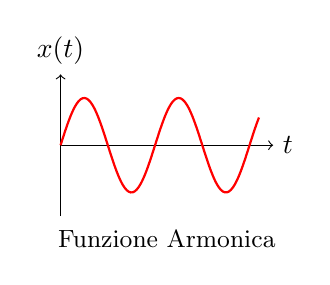
\begin{tikzpicture}[scale=0.6]
            \draw[->] (0,0) -- (4.5,0) node[right] {$t$};
            \draw[->] (0,-1.5) -- (0,1.5) node[above] {$x(t)$};
            \draw[thick, red, smooth, domain=0:4.2, samples=100] plot (\x, {sin(\x*180/1)});
            \node[below, font=\small] at (2.25,-1.6) {Funzione Armonica};
        \end{tikzpicture}
    \end{minipage}
\end{figure}

\begin{itemize}
    \item \textbf{Funzione Periodica}: Una funzione che si ripete identica dopo un periodo $T$ (es. l'onda quadra a sinistra). Qualunque forma è ammessa purché $f(t) = f(t+T)$.
    \item \textbf{Funzione Armonica}: Una specifica funzione periodica con andamento sinusoidale ($A\sin(\omega t + \phi)$). Matematicamente, è legata a una forza di richiamo proporzionale allo spostamento.
\end{itemize}

\begin{definizione}{Moto Armonico Semplice (MAS)}
Il moto armonico è un moto la cui legge oraria è una \textbf{funzione armonica}. Esso deve soddisfare l'equazione differenziale specifica:
\begin{equation}
    \ddot{x}(t) = -\omega^2 x(t)
\end{equation}
Tale equazione indica che in ogni istante l'accelerazione è proporzionale allo spostamento e rivolta verso la posizione di equilibrio.
\end{definizione}

\begin{osservazione}{Determinismo e Teorema di Cauchy}
Per determinare completamente l'evoluzione di un moto armonico, non basta l'equazione differenziale; è necessario conoscere le \textbf{condizioni iniziali} ($x_0, v_0$). Secondo il \textbf{Teorema di Cauchy} (esistenza e unicità), date tali condizioni, la soluzione è univocamente determinata.
\end{osservazione}

\subsection{Legge Oraria}
La soluzione dell'equazione differenziale è del tipo:
\begin{equation}
    x(t) = A \sin(\omega t + \phi)
\end{equation}
Dove:
\begin{itemize}
    \item $[A]$: \textbf{Ampiezza} dell'oscillazione (massimo spostamento dalla posizione di equilibrio).
    \item $[\omega]$: \textbf{Pulsazione} del moto (rad/s).
    \item $[\phi]$: \textbf{Fase iniziale} (o sfasamento rispetto a $\omega t$).
    \item $x(t)$: \textbf{Elongazione} al tempo $t$.
\end{itemize}

Poiché il moto è periodico, definiamo:
\begin{itemize}
    \item \textbf{Periodo} $[T]$: Il tempo impiegato per compiere un'oscillazione completa $[s]$.
    \[ T = \frac{2\pi}{\omega} \]
    \item \textbf{Frequenza} $[f]$: Numero di oscillazioni compiute nell'unità di tempo $[Hz]$ ($s^{-1}$).
    \[ f = \frac{1}{T} = \frac{\omega}{2\pi} \]
\end{itemize}

\subsection{Velocità e Accelerazione}
Derivando la legge oraria otteniamo:
\begin{align}
    v(t) &= \frac{dx}{dt} = A\omega \cos(\omega t + \phi) \\
    a(t) &= \frac{dv}{dt} = -A\omega^2 \sin(\omega t + \phi)
\end{align}
Osserviamo che:
\[ a(t) = -\omega^2 [A \sin(\omega t + \phi)] = -\omega^2 x(t) \]
Ritroviamo così la caratteristica fondamentale: l'accelerazione è proporzionale a $-x(t)$.

\subsection{Forme Alternative}
Le leggi orarie si possono trovare scritte anche in modi equivalenti, sfruttando le proprietà trigonometriche (come $\sin(\theta) = \cos(90^\circ - \theta)$):
\begin{itemize}
    \item $x(t) = A \cos(\omega t + \psi)$ (dove $\psi \neq \phi$)
    \item Combinazione lineare: $x(t) = \alpha \sin(\omega t) + \beta \cos(\omega t)$
\end{itemize}
Esistono correlazioni tra i coefficienti per passare da una forma all'altra:
\[ A = \sqrt{\alpha^2 + \beta^2}, \quad \tan(\phi) = \frac{\beta}{\alpha} \]

\paragraph{Nota Geometrica:}
Si può vedere il moto armonico semplice come la \textbf{proiezione di un moto circolare uniforme} su un diametro (una retta).

\section{Moto Smorzato Esponenzialmente}
È un moto la cui velocità decresce esponenzialmente nel tempo.
Le leggi orarie sono:
\[ x(t) = A \left(1 - e^{-\frac{t}{\tau}}\right), \quad v(t) = \frac{A}{\tau} e^{-\frac{t}{\tau}}, \quad a(t) = -\frac{A}{\tau^2} e^{-\frac{t}{\tau}} \]
Dove $\tau$ è la costante di tempo e $A$ è il valore asintotico della posizione (la quota a cui tende).

\begin{figure}[h]
    \centering
    \begin{tikzpicture}[scale=0.9]
        \draw[->] (0,0) -- (5,0) node[right] {$t$};
        \draw[->] (0,0) -- (0,3) node[above] {$x(t)$};
        \draw[dashed] (0,2.5) -- (5,2.5) node[right] {$A$};
        \draw[thick, blue] plot[domain=0:4.8, samples=100] (\x, {2.5*(1 - exp(-\x))});
    \end{tikzpicture}
    \caption{Andamento della posizione nel moto smorzato: tende asintoticamente ad $A$.}
\end{figure}

\section{Moto dei Gravi}
È un moto rettilineo uniformemente accelerato con accelerazione costante $\vec{a} = -\vec{g}$ (diretta verso il basso), dove $g \approx 9.81 \, m/s^2$.

\subsection{Caduta da $y_0 \neq 0$}
Consideriamo un corpo lasciato cadere da un'altezza $y_0$ con velocità iniziale nulla ($v_0 = 0$).

Le equazioni sono:
\begin{align*}
    a(t) &= -g \\
    v(t) &= -g(t - t_0) \\
    y(t) &= y(t_0) - \frac{1}{2}g(t - t_0)^2
\end{align*}

Possiamo calcolare il \textbf{tempo di caduta} $t_f$ imponendo $y(t_f) = 0$:
\[ t_f = t_0 + \sqrt{\frac{2y_0}{g}} \]

La \textbf{velocità finale} (di impatto) sarà:
\[ v_f = - \sqrt{2y_0 g} \]
(negativa perché il vettore velocità è diretto verso il basso, concorde a $\vec{g}$).

\begin{center}
    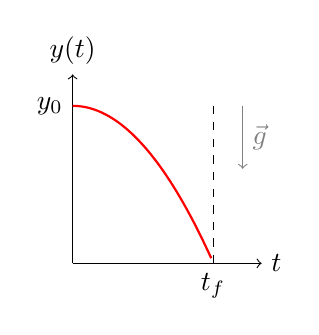
\begin{tikzpicture}[scale=0.8]
        \draw[->] (0,0) -- (3,0) node[right] {$t$};
        \draw[->] (0,0) -- (0,3) node[above] {$y(t)$};
        \draw[thick, red] plot[domain=0:2.2, samples=50] (\x, {2.5 - 0.5*\x*\x});
        \node[left] at (0,2.5) {$y_0$};
        \draw[dashed] (2.23,0) -- (2.23, 2.5); % impact time
        \node[below] at (2.23,0) {$t_f$};
        \draw[->, gray] (2.7, 2.5) -- (2.7, 1.5) node[midway, right] {$\vec{g}$};
    \end{tikzpicture}
\end{center}

\subsection{Lancio verso l'alto da $y_0 = 0$}
Consideriamo un corpo lanciato verso l'alto con velocità iniziale $v(t_0) > 0$.

Le equazioni sono:
\begin{align*}
    v(t) &= v(t_0) - g(t - t_0) \\
    y(t) &= v(t_0)(t - t_0) - \frac{1}{2}g(t - t_0)^2
\end{align*}

\textbf{Analisi del moto:}
\begin{itemize}
    \item $v(t) > 0$ nella fase di ascesa.
    \item $v(t) < 0$ nella fase di discesa.
    \item Quando $v(t) = 0$, il corpo raggiunge la \textbf{quota massima} $y_m$. Questo avviene all'istante:
    \[ t_{\text{apice}} = \frac{v(t_0)}{g} \]
\end{itemize}
Sostituendo il tempo nell'equazione della posizione, otteniamo la quota massima:
\[ y_m = \frac{v(t_0)^2}{2g} \]

Il tempo totale di volo $t_f$ (per tornare a terra) è il doppio del tempo di salita:
\[ t_f = t_0 + \frac{2v(t_0)}{g} \]

\begin{center}
    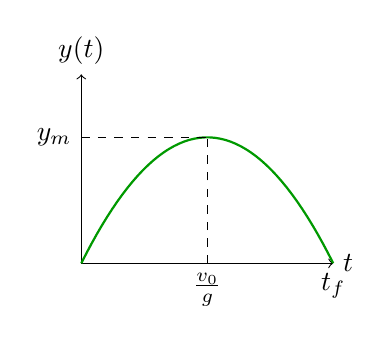
\begin{tikzpicture}[scale=0.8]
        \draw[->] (0,0) -- (4,0) node[right] {$t$};
        \draw[->] (0,0) -- (0,3) node[above] {$y(t)$};
        % Parabola starting at 0, peak at x=2, y=2, landing at x=4
        \draw[thick, green!60!black] plot[domain=0:4, samples=50] (\x, {2*\x - 0.5*\x*\x});
        
        \draw[dashed] (0,2) -- (2,2);
        \node[left] at (0,2) {$y_m$};
        
        \draw[dashed] (2,0) -- (2,2);
        \node[below] at (2,0) {$\frac{v_0}{g}$};
        
        \node[below] at (4,0) {$t_f$};
    \end{tikzpicture}
\end{center}

\section{Moto Parabolico}
Il moto parabolico è un moto in due dimensioni, composto dalla sovrapposizione di due moti indipendenti:
\begin{itemize}
    \item \textbf{Asse x}: Moto rettilineo uniforme ($a_x = 0$) $\Rightarrow v_x = \text{costante}$.
    \item \textbf{Asse y}: Moto uniformemente accelerato ($a_y = -g = -9.81 \, m/s^2$).
\end{itemize}

\subsection{Lancio con $\theta = 0^\circ$ (Lancio Orizzontale)}
Consideriamo un corpo lanciato orizzontalmente da un'altezza $y_0$ con velocità $v_0$.
In questo caso, l'angolo iniziale è nullo, quindi:
\[ v_{0x} = v_0 \cos(0^\circ) = v_0, \quad v_{0y} = v_0 \sin(0^\circ) = 0 \]

\textbf{Equazioni della velocità:}
\[
\begin{cases}
    v_x(t) = v_0 \\
    v_y(t) = -gt
\end{cases}
\]

\textbf{Leggi orarie:}
\[
\begin{cases}
    x(t) = v_0 t \\
    y(t) = y_0 - \frac{1}{2} g t^2
\end{cases}
\]

Il corpo atterra quando $y(t_f) = 0$.
\begin{itemize}
    \item \textbf{Tempo di caduta}: $t_f = \sqrt{\frac{2y_0}{g}}$
    \item \textbf{Gittata} ($x_f$): Sostituendo $t_f$ in $x(t)$:
    \[ x_f = v_0 \sqrt{\frac{2y_0}{g}} \]
    \item \textbf{Angolo finale d'impatto} $\theta_f$:
    \[ \tan \theta_f = \frac{v_y(t_f)}{v_x(t_f)} = \frac{-g t_f}{v_0} = \frac{-\sqrt{2y_0 g}}{v_0} \]
    \item \textbf{Velocità d'impatto verticale}: $v_{yf} = - \sqrt{2y_0 g}$
\end{itemize}

\begin{center}
    \begin{tikzpicture}[scale=0.8]
        \draw[->] (0,0) -- (4,0) node[right] {$x(t)$};
        \draw[->] (0,0) -- (0,3) node[above] {$y(t)$};
        
        \node[left] at (0,2.5) {$y_0$};
        \draw[dashed] (0,2.5) -- (4,2.5);
        \draw[->, thick] (0,2.5) -- (1,2.5) node[above] {$\vec{v}_0$};
        
        % Parabola starting at (0, 2.5) going down
        \draw[thick, blue] plot[domain=0:2.25, samples=50] (\x, {2.5 - 0.49*\x*\x});
        
        \node[below] at (2.25,0) {$x_f$};
    \end{tikzpicture}
\end{center}

\subsection{Lancio con \texorpdfstring{$\theta \neq 0^\circ$}{theta != 0} (Lancio Obliquo)}
Il corpo viene lanciato con una velocità iniziale $v_0$ che forma un angolo $\theta$ con l'orizzontale.
\[ v_{0x} = v_0 \cos\theta, \quad v_{0y} = v_0 \sin\theta \]

\textbf{Equazioni della velocità:}
\[
\begin{cases}
    v_x(t) = v_{0x} \quad (\text{costante}) \\
    v_y(t) = v_{0y} - gt
\end{cases}
\]

\textbf{Leggi orarie:}
\[
\begin{cases}
    x(t) = x_0 + v_{0x} t \\
    y(t) = y_0 + v_{0y} t - \frac{1}{2} g t^2
\end{cases}
\]

\textbf{Proprietà del moto:}
\begin{itemize}
    \item \textbf{Direzione istantanea}: $\tan \theta(t) = \frac{v_y(t)}{v_x(t)}$.
    \item \textbf{Quota Massima} ($y_m$): Si raggiunge quando $v_y = 0$, ovvero a $t = \frac{v_{0y}}{g}$.
    \[ y_m = y_0 + \frac{v_{0y}^2}{2g} = y_0 + \frac{(v_0 \sin\theta)^2}{2g} \]
    \item \textbf{Tempo di volo} (atterraggio alla stessa quota $y_0$): $t_f = \frac{2v_{0y}}{g}$.
    \item \textbf{Gittata} ($x_m$): Distanza orizzontale percorsa.
    \[ x_m = v_{0x} t_f = \frac{v_0^2 \sin(2\theta)}{g} \]
    Nota: La gittata è massima per $\theta = 45^\circ$ ($\sin 90^\circ = 1$) ed è uguale per angoli complementari ($\theta$ e $90^\circ - \theta$).
\end{itemize}

\begin{center}
    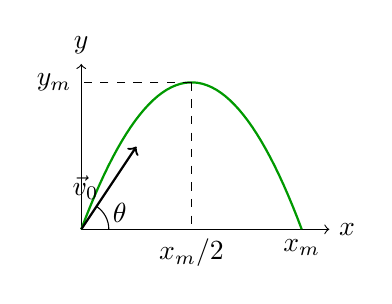
\begin{tikzpicture}[scale=0.7]
        \draw[->] (0,0) -- (4.5,0) node[right] {$x$};
        \draw[->] (0,0) -- (0,3) node[above] {$y$};
        
        % Parabola
        \draw[thick, green!60!black] plot[domain=0:4, samples=50] (\x, {-\x*(\x-4)/1.5});
        
        % Vector v0
        \draw[->, thick] (0,0) -- (1, 1.5) node[midway, left] {$\vec{v}_0$};
        \draw (0.5,0) arc (0:56:0.5);
        \node at (0.7, 0.3) {$\theta$};
        
        \draw[dashed] (2, 2.66) -- (0, 2.66) node[left] {$y_m$};
        \draw[dashed] (2, 2.66) -- (2, 0) node[below] {$x_m/2$};
        \node[below] at (4,0) {$x_m$};
    \end{tikzpicture}
\end{center}

\subsubsection{Equazione della Traiettoria}
Eliminando il tempo $t = x/v_{0x}$ dalle leggi orarie (ponendo $x_0=y_0=0$), otteniamo la relazione tra $y$ e $x$:
\[ y(x) = x \tan\theta - \frac{g}{2v_0^2 \cos^2\theta} x^2 \]
Questa è l'equazione di una parabola con concavità verso il basso.

\subsubsection{Geometria della Sicurezza}
\begin{itemize}
    \item \textbf{Luogo dei vertici}: Le coordinate dei vertici delle parabole al variare di $\theta$ descrivono un'ellisse:
    \[ x_v^2 + 4y_v^2 = \frac{2v_0^2}{g} y_v \]
    \item \textbf{Parabola di Sicurezza}: L'inviluppo di tutte le possibili traiettorie (al variare di $\theta$ con $v_0$ fissato) definisce la regione di spazio raggiungibile dal proiettile. Questa regione è delimitata dalla \textbf{parabola di sicurezza}.
\end{itemize}

\section{Moto Circolare Uniforme (MCU)}
Il moto circolare è caratterizzato da alcune nuove grandezze vettoriali:
\begin{itemize}
    \item $\vec{\omega}$: \textbf{Velocità Angolare}.
    \item $\vec{a}_n$: \textbf{Accelerazione Centripeta} (o Normale).
    \item $\vec{a}_t$: \textbf{Accelerazione Tangenziale} (presente solo se il moto non è uniforme).
    \item $\vec{\alpha}$: \textbf{Accelerazione Angolare} (presente solo se il moto non è uniforme).
\end{itemize}

\begin{definizione}{Componenti dell'Accelerazione}
\begin{itemize}
    \item \textbf{Accelerazione Centripeta / Normale} ($\vec{a}_n$): Esprime la \textbf{variazione di direzione} della velocità. È sempre presente in un moto curvilineo e punta verso il centro di curvatura.
    \item \textbf{Accelerazione Tangenziale} ($\vec{a}_t$): Esprime la \textbf{variazione di modulo} della velocità. È parallela alla velocità istantanea.
    \item \textbf{Accelerazione Angolare} ($\vec{\alpha}$): Derivata della velocità angolare rispetto al tempo ($\vec{\alpha} = d\vec{\omega}/dt$).
\end{itemize}
\end{definizione}

\begin{figure}[h]
    \centering
    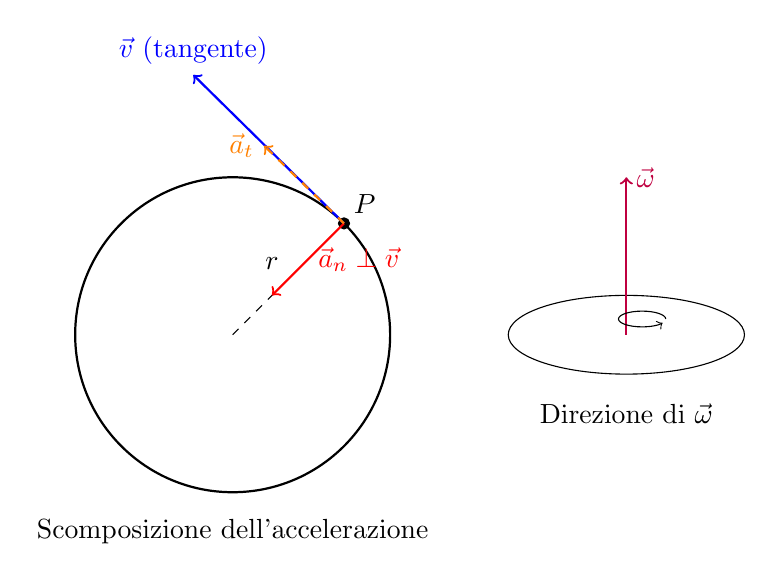
\begin{tikzpicture}[scale=1]
        % Circle
        \draw[thick] (0,0) circle (2cm);
        \draw[dashed] (0,0) -- (1.414, 1.414) node[midway, above left] {$r$};
        \filldraw (1.414, 1.414) circle (2pt) node[above right] {$P$};
        
        % Vectors
        \draw[->, thick, blue] (1.414, 1.414) -- (-0.5, 3.3) node[above] {$\vec{v}$ (tangente)};
        \draw[->, thick, red] (1.414, 1.414) -- (0.5, 0.5) node[midway, right] {$\vec{a}_n \perp \vec{v}$};
        
        % Tangential acceleration (dashed imaginary for MCU)
        \draw[->, thick, orange, dashed] (1.414, 1.414) -- (0.4, 2.4) node[left] {$\vec{a}_t$};
        
        \node at (0,-2.5) {Scomposizione dell'accelerazione};
        
        % Angular velocity 3D illusion
        \begin{scope}[xshift=5cm]
            \draw (0,0) ellipse (1.5cm and 0.5cm);
            \draw[->, thick, purple] (0,0) -- (0, 2) node[right] {$\vec{\omega}$};
            \draw[->] (0.5, 0.2) arc (0:330:0.3 and 0.1);
            \node at (0,-1) {Direzione di $\vec{\omega}$};
        \end{scope}
    \end{tikzpicture}
    \caption{Cinematica del moto circolare.}
\end{figure}

\subsection{Relazioni Fondamentali (MCU)}
Nel moto circolare uniforme ($|v|=$ cost, $\alpha=0$), le grandezze sono così relazionate:
\begin{itemize}
    \item Velocità tangenziale: $|v| = \omega r$
    \item Periodo: $T = \frac{2\pi}{\omega} = \frac{2\pi r}{v}$
    \item Frequenza: $f = \frac{1}{T}$
    \item Velocità angolare: $|\omega| = \frac{2\pi}{T} = 2\pi f$
    \item Modulo accelerazione centripeta: $a_c = \omega^2 r = \frac{v^2}{r}$
\end{itemize}

\clearpage
\section{Approfondimento: Sistemi di Riferimento e Algebra dei Versori}
Prima di analizzare nel dettaglio la dinamica del moto circolare, è fondamentale definire formalmente i sistemi di coordinate e le proprietà dei versori (vettori unitari) associati.

\subsection{Versori e Derivazione Temporale}
Un sistema di riferimento è definito da un'origine $O$ e da una base di versori. La caratteristica cruciale per la cinematica è se questi versori sono \textbf{fissi} o \textbf{mobili} nel tempo.

\subsubsection{Coordinate Cartesiane $(x, y)$}
La base è costituita dai versori $\{\hat{x}, \hat{y}\}$:
\begin{itemize}
    \item Hanno modulo unitario ($|\hat{x}| = |\hat{y}| = 1$) e sono ortogonali.
    \item Hanno \textbf{direzione e verso fissi} nello spazio.
\end{itemize}
Pertanto, la loro derivata rispetto al tempo è nulla:
\[ \frac{d\hat{x}}{dt} = \vec{0}, \quad \frac{d\hat{y}}{dt} = \vec{0} \]
Il vettore posizione si scrive come: $\vec{r}(t) = x(t)\hat{x} + y(t)\hat{y}$.

\begin{center}
\begin{tikzpicture}[scale=1.5]
    % Assi
    \draw[->] (-2.5,0) -- (2.5,0) node[right] {$x$};
    \draw[->] (0,-2.5) -- (0,2.5) node[above] {$y$};
    
    % Traiettoria Circolare (MCU)
    \draw[thick, gray, dashed] (0,0) circle (2cm);
    
    % Versori fissi origin
    \draw[->, thick, red] (0,0) -- (1,0) node[below] {$\hat{x}$};
    \draw[->, thick, red] (0,0) -- (0,1) node[left] {$\hat{y}$};
    
    % Punto P a 45 gradi su r=2 -> P(1.414, 1.414)
    \filldraw (1.414, 1.414) circle (1.5pt) node[above right] {$P(x,y)$};
    \draw[dashed] (1.414,0) node[below] {$x$} -- (1.414,1.414) -- (0,1.414) node[left] {$y$};
    
    % Vettore posizione
    \draw[->, thick, blue] (0,0) -- (1.414, 1.414) node[midway, above left] {$\vec{r}(t)$};
\end{tikzpicture}
\end{center}

\subsubsection{Coordinate Polari Piane $(\rho, \theta)$}
La base è costituita dai versori $\{\hat{\rho}, \hat{\theta}\}$:
\begin{itemize}
    \item $\hat{\rho}$: Versore \textbf{radiale}, diretto dall'origine verso il punto $P$.
    \item $\hat{\theta}$: Versore \textbf{trasverso} (o azimutale), perpendicolare a $\hat{\rho}$ nel verso di crescita di $\theta$.
\end{itemize}

\begin{center}
\begin{tikzpicture}[scale=1.5]
    % Assi riferimento
    \draw[->, gray] (-2.5,0) -- (2.5,0) node[right] {$x$};
    \draw[->, gray] (0,-2.5) -- (0,2.5) node[above] {$y$};
    
    % Traiettoria Circolare (MCU)
    \draw[thick, gray, dashed] (0,0) circle (2cm);
    
    % Punto P
    \filldraw (1.414, 1.414) circle (1.5pt) node[above left] {$P(\rho,\theta)$};
    
    % Vettore rho (coincide con il raggio)
    \draw[->, thick, blue] (0,0) -- (1.414, 1.414) node[midway, below right] {$\vec{\rho}$};
    \draw[dashed, gray] (1.414,1.414) -- (2.121, 2.121); % Prolungamento
    
    % Angolo theta
    \draw (0.8,0) arc (0:45:0.8);
    \node at (1, 0.4) {$\theta$};
    
    % Versori mobili in P
    \draw[->, thick, red] (1.414, 1.414) -- (2.121, 2.121) node[right] {$\hat{\rho}$};
    \draw[->, thick, red] (1.414, 1.414) -- (0.707, 2.121) node[above] {$\hat{\theta}$};
    
    % Angolo retto tra i versori
    \draw (1.556, 1.556) -- (1.414, 1.697) -- (1.273, 1.556);
\end{tikzpicture}
\end{center}

Possiamo esprimerli in funzione della base cartesiana (fissa):
\[ \hat{\rho} = \cos\theta \, \hat{x} + \sin\theta \, \hat{y} \]
\[ \hat{\theta} = -\sin\theta \, \hat{x} + \cos\theta \, \hat{y} \]

\begin{teorema}{Formule di Poisson nel Piano}
Le derivate temporali dei versori polari mobili $\{\hat{\rho}, \hat{\theta}\}$ si esprimono in funzione della velocità angolare $\dot{\theta}$:
\begin{equation}
    \frac{d\hat{\rho}}{dt} = \dot{\theta} \hat{\theta}, \quad \frac{d\hat{\theta}}{dt} = -\dot{\theta} \hat{\rho}
\end{equation}
\end{teorema}
Queste relazioni (Formule di Poisson nel piano) sono fondamentali per derivare velocità e accelerazione in coordinate polari.

\subsubsection{Coordinate Intrinseche $(s)$}
La base è locale alla traiettoria, definita dai versori $\{\hat{\tau}, \hat{n}\}$:
\begin{itemize}
    \item $\hat{\tau}$: Versore \textbf{tangente}, parallelo alla velocità.
    \item $\hat{n}$: Versore \textbf{normale}, diretto verso il centro di curvatura locale.
\end{itemize}

\begin{center}
\begin{tikzpicture}[scale=1.5]
    % Traiettoria (Circolare per MCU)
    \draw[thick, gray, dashed] (0,0) circle (2cm);
    
    % Centro di curvatura (origine)
    \filldraw (0, 0) circle (1pt) node[below] {$C$};
    
    % Punto P a 45 gradi su r=2
    \filldraw (1.414, 1.414) circle (1.5pt) node[above right] {$P$};
    
    % Raggio di curvatura
    \draw[dashed] (0, 0) -- (1.414, 1.414) node[midway, left] {$R$};
    
    % Versori mobili in P
    % n punta verso il centro C (origine), theta/tau è radente
    \draw[->, thick, red] (1.414, 1.414) -- (0.707, 2.121) node[above left] {$\hat{\tau}$};
    \draw[->, thick, red] (1.414, 1.414) -- (0.707, 0.707) node[below right] {$\hat{n}$};
    
    % Vettore velocità (parallelo a tau)
    \draw[->, thick, blue] (1.414, 1.414) -- (0, 2.828) node[left] {$\vec{v}$};
\end{tikzpicture}
\end{center}

Nel caso del moto circolare, valgono le seguenti identificazioni geometriche con i versori polari:
\[ \hat{\tau} \equiv \hat{\theta}, \quad \hat{n} \equiv -\hat{\rho} \]
La relazione fondamentale è $\frac{d\hat{\tau}}{dt} = \frac{v}{R} \hat{n}$ (dove $R$ è il raggio di curvatura).

\section{Analisi del Moto Circolare nei vari Sistemi}
Applichiamo ora l'algebra dei versori appena definita al caso specifico del moto circolare di raggio $R$ costante.

\subsection{Caso 1: Coordinate Cartesiane}
Descriviamo il punto $P$ tramite la proiezione sugli assi $x$ e $y$.
Sia $\theta(t) = \omega t + \phi_0$ la legge oraria angolare.
\[
\begin{cases}
    x(t) = R \cos(\omega t + \phi_0) \\
    y(t) = R \sin(\omega t + \phi_0)
\end{cases}
\]

\textbf{Velocità}: Deriviamo le componenti rispetto al tempo ($\dot{x}, \dot{y}$):
\[
\begin{cases}
    v_x = \dot{x} = -R\omega \sin(\omega t + \phi_0) = -\omega y \\
    v_y = \dot{y} = R\omega \cos(\omega t + \phi_0) = \omega x
\end{cases}
\]

\textbf{Accelerazione}: Deriviamo nuovamente ($\ddot{x}, \ddot{y}$):
\[
\begin{cases}
    a_x = \ddot{x} = -R\omega^2 \cos(\omega t + \phi_0) = -\omega^2 x \\
    a_y = \ddot{y} = -R\omega^2 \sin(\omega t + \phi_0) = -\omega^2 y
\end{cases}
\]
Notiamo che $\vec{a} = a_x \hat{x} + a_y \hat{y} = -\omega^2 (x\hat{x} + y\hat{y}) = -\omega^2 \vec{r}$.
Questo conferma che l'accelerazione è \textbf{centripeta} (opposta al raggio vettore) e proporzionale al quadrato della velocità angolare. Inoltre, le proiezioni sugli assi sono \textbf{moti armonici} di pulsazione $\omega$.

\subsection{Caso 2: Coordinate Polari}
Il vettore posizione è definito semplicemente da:
\[ \vec{r}(t) = \rho(t) \hat{\rho} \]
Nel moto circolare, il raggio è costante $\rho(t) = R$, quindi $\dot{\rho} = 0, \ddot{\rho} = 0$.
L'angolo varia come $\theta(t)$, con velocità angolare $\dot{\theta} = \omega$ e accelerazione angolare $\ddot{\theta} = \alpha$.

\textbf{Velocità}: Deriviamo $\vec{r}$ usando la regola del prodotto:
\[ \vec{v} = \frac{d}{dt}(R \hat{\rho}) = \dot{R}\hat{\rho} + R\frac{d\hat{\rho}}{dt} \]
Poiché $\dot{R}=0$ e $\frac{d\hat{\rho}}{dt} = \dot{\theta}\hat{\theta} = \omega \hat{\theta}$:
\[ \vec{v} = R\omega \hat{\theta} \]
(La velocità è puramente tangenziale, diretta lungo $\hat{\theta}$).

\textbf{Accelerazione}: Deriviamo $\vec{v}$:
\[ \vec{a} = \frac{d}{dt}(R\omega \hat{\theta}) = R\dot{\omega}\hat{\theta} + R\omega\frac{d\hat{\theta}}{dt} \]
Ricordando che $\dot{\omega} = \alpha$ e $\frac{d\hat{\theta}}{dt} = -\omega \hat{\rho}$:
\[ \vec{a} = R\alpha \hat{\theta} - R\omega^2 \hat{\rho} \]
Abbiamo ottenuto le due componenti vettoriali in modo formale:
\begin{itemize}
    \item \textbf{Componente Tangenziale} ($\vec{a}_t = R\alpha \hat{\theta}$): Dipende da $\alpha$. Se il moto è uniforme ($\alpha=0$), questa componente è nulla.
    \item \textbf{Componente Centripeta} ($\vec{a}_n = -R\omega^2 \hat{\rho}$): Sempre presente, diretta lungo $-\hat{\rho}$ (verso il centro).
\end{itemize}

\subsection{Caso 3: Coordinate Intrinseche}
In questo sistema, i versori sono definiti localmente sulla curva. Per il moto circolare valgono le identità:
\[ \hat{\tau} \equiv \hat{\theta}, \quad \hat{n} \equiv -\hat{\rho} \]

Sappiamo che:
\[ \vec{v} = v \hat{\tau} \]
Deriviamo rispetto al tempo:
\[ \vec{a} = \frac{dv}{dt}\hat{\tau} + v\frac{d\hat{\tau}}{dt} \]
Usando la relazione geometrica $\frac{d\hat{\tau}}{dt} = \frac{v}{R}\hat{n}$:
\[ \vec{a} = \frac{dv}{dt}\hat{\tau} + \frac{v^2}{R}\hat{n} \]

Sostituendo i versori intrinseci con quelli polari:
\[ \vec{a} = (R\alpha)\hat{\theta} + \frac{(R\omega)^2}{R}(-\hat{\rho}) = R\alpha \hat{\theta} - R\omega^2 \hat{\rho} \]

\clearpage
\section{Moti Curvilinei Generali in Coordinate Polari}
Estendiamo l'analisi al caso più generale di un \textbf{moto curvilineo}, dove il raggio di curvatura non è necessariamente costante (quindi $\rho = \rho(t)$ varia nel tempo). Vogliamo derivare l'espressione completa di velocità e accelerazione in coordinate polari piane $(\rho, \theta)$.

\subsection{Posizione e Velocità}
Il vettore posizione è:
\[ \vec{r}(t) = \rho(t) \hat{\rho}(t) \]
Derivandolo rispetto al tempo per ottenere la velocità, dobbiamo applicare la regola del prodotto (poiché sia il modulo $\rho$ che il versore $\hat{\rho}$ variano):
\[ \vec{v} = \frac{d\vec{r}}{dt} = \frac{d\rho}{dt}\hat{\rho} + \rho\frac{d\hat{\rho}}{dt} \]
Ricordando la formula di Poisson $\frac{d\hat{\rho}}{dt} = \dot{\theta}\hat{\theta}$:
\[ \vec{v} = \dot{\rho}\hat{\rho} + \rho\dot{\theta}\hat{\theta} \]
Possiamo identificare i due termini (anche quelli nascosti dal foglio verde nella figura originale):
\begin{itemize}
    \item $v_\rho = \dot{\rho}$: \textbf{Velocità Radiale} (dovuta alla variazione della distanza dall'origine).
    \item $v_\theta = \rho\dot{\theta}$: \textbf{Velocità Trasversa/Angolare} (dovuta alla rotazione del raggio vettore).
\end{itemize}

\subsection{Accelerazione: Derivazione Completa}
Per ottenere l'accelerazione, deriviamo nuovamente la velocità:
\[ \vec{a} = \frac{d}{dt}(\dot{\rho}\hat{\rho} + \rho\dot{\theta}\hat{\theta}) \]
Applichiamo la derivata ai due termini separatamente:
\begin{enumerate}
    \item Primo termine ($\dot{\rho}\hat{\rho}$):
    \[ \frac{d}{dt}(\dot{\rho}\hat{\rho}) = \ddot{\rho}\hat{\rho} + \dot{\rho}\frac{d\hat{\rho}}{dt} = \ddot{\rho}\hat{\rho} + \dot{\rho}\dot{\theta}\hat{\theta} \]
    \item Secondo termine ($\rho\dot{\theta}\hat{\theta}$), regola del prodotto a tre fattori ($fgh \to f'gh + fg'h + fgh'$):
    \[ \frac{d}{dt}(\rho\dot{\theta}\hat{\theta}) = \dot{\rho}\dot{\theta}\hat{\theta} + \rho\ddot{\theta}\hat{\theta} + \rho\dot{\theta}\frac{d\hat{\theta}}{dt} \]
    Ricordando che $\frac{d\hat{\theta}}{dt} = -\dot{\theta}\hat{\rho}$, diventa:
    \[ = \dot{\rho}\dot{\theta}\hat{\theta} + \rho\ddot{\theta}\hat{\theta} - \rho\dot{\theta}^2\hat{\rho} \]
\end{enumerate}

Sommando tutti i contributi e raggruppando per versori:
\[ \vec{a} = (\ddot{\rho}\hat{\rho} + \dot{\rho}\dot{\theta}\hat{\theta}) + (\dot{\rho}\dot{\theta}\hat{\theta} + \rho\ddot{\theta}\hat{\theta} - \rho\dot{\theta}^2\hat{\rho}) \]

\begin{teorema}{Accelerazione in Coordinate Polari}
L'espressione completa dell'accelerazione per un moto curvilineo generale $\vec{r} = \rho \hat{\rho}$ è:
\begin{equation}
    \vec{a} = (\ddot{\rho} - \rho \dot{\theta}^2)\hat{\rho} + (2\dot{\rho}\dot{\theta} + \rho \ddot{\theta}) \hat{\theta}
\end{equation}
Identifichiamo i 4 contributi fisici:
\begin{itemize}
    \item $\ddot{\rho}$: \textbf{Accelerazione Radiale}.
    \item $-\rho \dot{\theta}^2$: \textbf{Accelerazione Centripeta}.
    \item $\rho \ddot{\theta}$: \textbf{Accelerazione Tangenziale}.
    \item $2\dot{\rho}\dot{\theta}$: \textbf{Accelerazione di Coriolis}.
\end{itemize}
\end{teorema}
